%!TEX root = ../thesis.tex
%*******************************************************************************
%****************************** Third Chapter **********************************
%*******************************************************************************
\chapter{Gamma Correction in Holographic Projection} \label{sec:Gamma Correction in Holographic Projection}

\graphicspath{{Chapter3/Figs/}}

\textit{Note: This Chapter is a continuation of my masters project in 2019-2020, which was unexpectedly terminated early by COVID-19. During my first year of PhD study, all measurements have been retaken for quantified analysis.}\\\\
In order to improve image quality of holographic projection, the idea of the gamma correction method arose to improve the contrast of the replay field. Every display has an inherent property known as the gamma value $\gamma$, which essentially describes the transfer function between input pixel value and output pixel energy\cite{Gonzalez2002}. Gamma correction is normally done via a look-up table or correction curve which allows the relationship between the input and output to be adjusted. In a computer-generated holographic projection system, the image is generated via diffraction of light from spatial light modulators. In this process, several factors contribute to non-linearities between the replay field and the target image. This section evaluates the gamma response of the overall system experimentally, and then applies a gamma correction method, with the aim of increasing the image quality of a holographic projection system. Both a notable increase in replay field quality alongside a significant reduction in mean squared error were observed, demonstrating the effectiveness of gamma correction in holographic projection.


\section{Experimental Setup}\label{sec:Experimental Setup}
\begin{figure}[H]
  \centering
  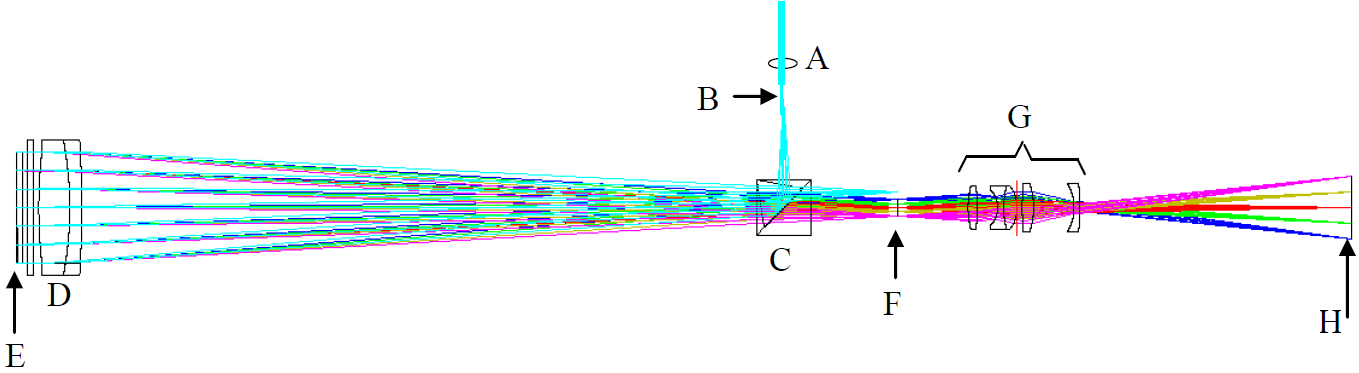
\includegraphics[width=1.0\textwidth]{projection_setup.png}
  \caption{Optical setup \cite{Freeman2009}}
  \label{fig:projection_setup}
\end{figure}

The holographic projector used in this experiment was a Fourier projection system developed by Freeman \cite{Freeman2009}, as shown in \cref{fig:projection_setup}. The design is consisted of a diode-pumped solid-state (DPSS) 532 nm 50mW laser source, focussed down by an aspheric singlet (A), the focus of which becomes the diffraction limited point source (B) for the projector. The beam then passes through a polarising beam splitter cube (C) to a collimating lens (D), which illuminates the SLM (E). The SLM is a binary phase SXGA-R2 ForthDD ferroelectric Liquid crystal on silicon (LCOS) micro-display with a refresh rate of 1440Hz, a pixel pitch of \SI{13.6}{\micro\metre} and a resolution of $1280\times1024$. An aperture at point (F) spatially filters out the other orders, leaving only one first order, which is then magnified up by a finite conjugate lens group (G) to produce an image, of the required size, on the screen (H). \cite{Freeman2009}

The holograms displayed on the SLM are generated using the one-step phase retrieval (OSPR) algorithm \cite{Cable2006} explained in \cref{sec:One Step Phase Retrieval (OSPR) Algorithm}, where each group of 24 individual, binary-phase holograms are encoded as the 8-bit reg, green, blue (RGB) channels of a 24-bit image to interface with the SLM driver electronics. The SLM displays each bit plane sequentially, with ones and zeros mapping to opposing phase modulations at each pixel. The images were captured using a Canon 550D camera with an EFS 18-55 mm lens. To ensure fair comparison, the camera was set to the same manual setting when comparing each pair of replay fields before and after gamma correction. The images captured were in 24-bit RGB colour, which were subsequently converted to grey-scale in 8-bit depth when calculating normalised mean squared error (NMSE).



\section{Determining the Gamma Correction Curve}\label{sec:Determining the gamma correction curve}

\begin{figure}[H]
  \centering
  \begin{subfigure}[c]{0.32\textwidth}
    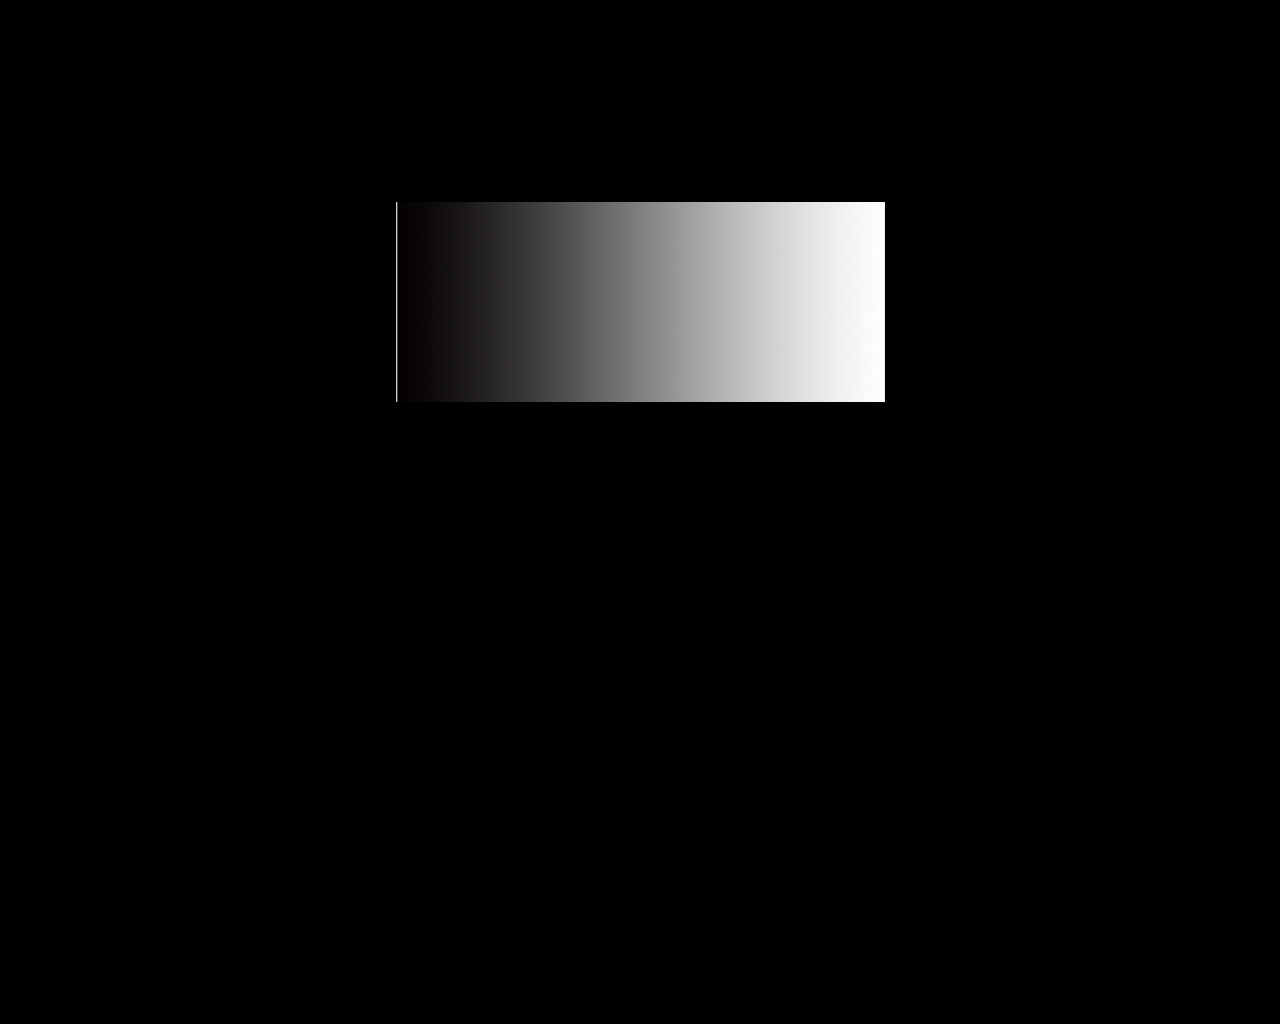
\includegraphics[width=\textwidth]{grey-scale-test.png}
    \caption{Input linear grey-scale ramp}\label{fig:grey-scale-test}
  \end{subfigure}
  \hfill
  \begin{subfigure}[c]{0.32\textwidth}
    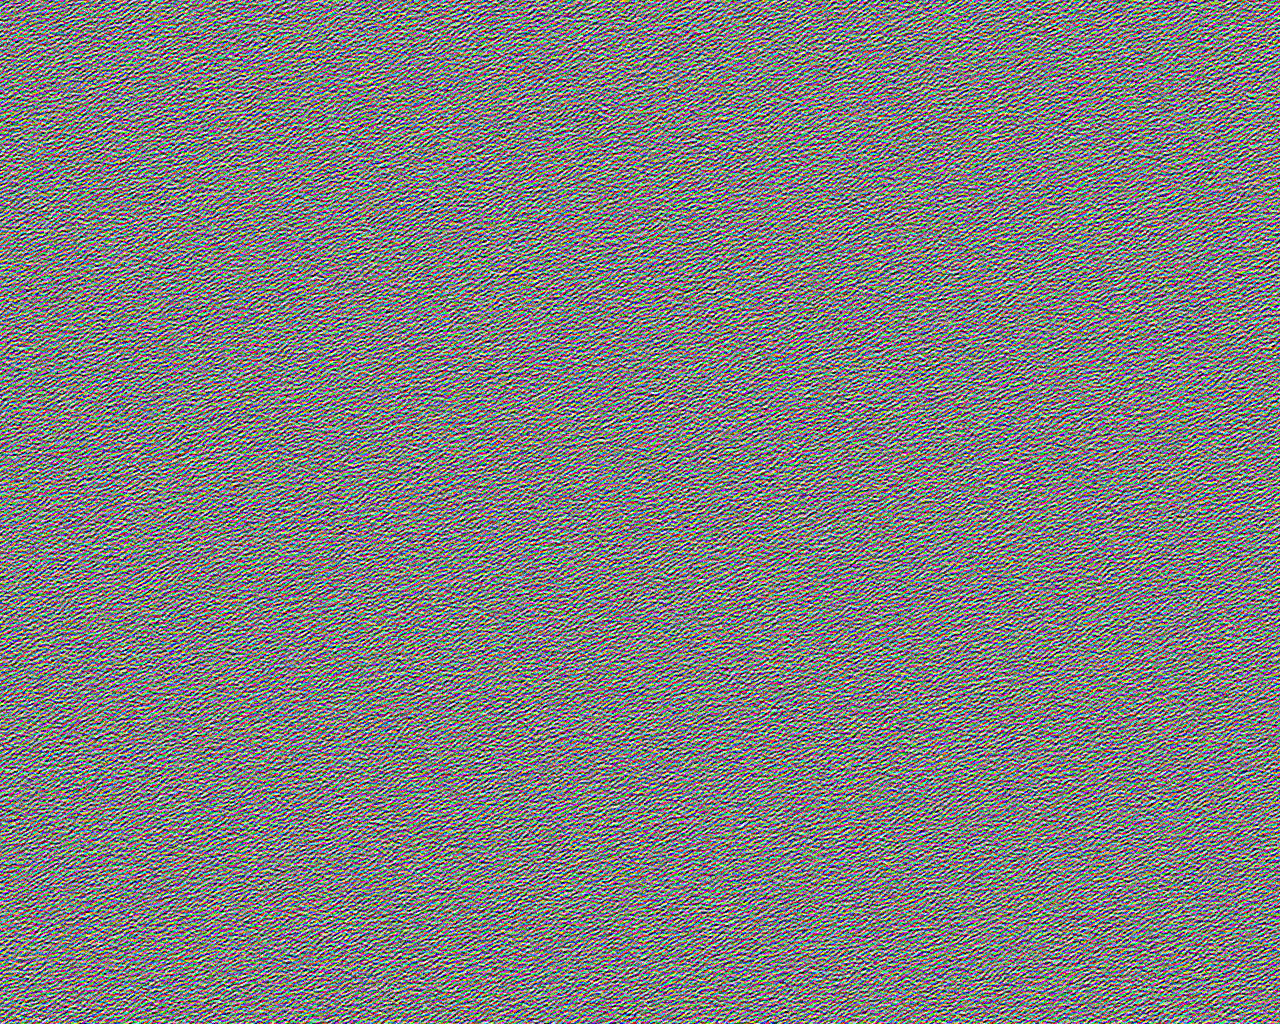
\includegraphics[width=\textwidth]{Holo_linear_ramp.png}
    \caption{CGH of \cref{fig:grey-scale-test}}\label{fig:Holo_linear_ramp}
  \end{subfigure}
  \hfill
  \begin{subfigure}[c]{0.32\textwidth}
    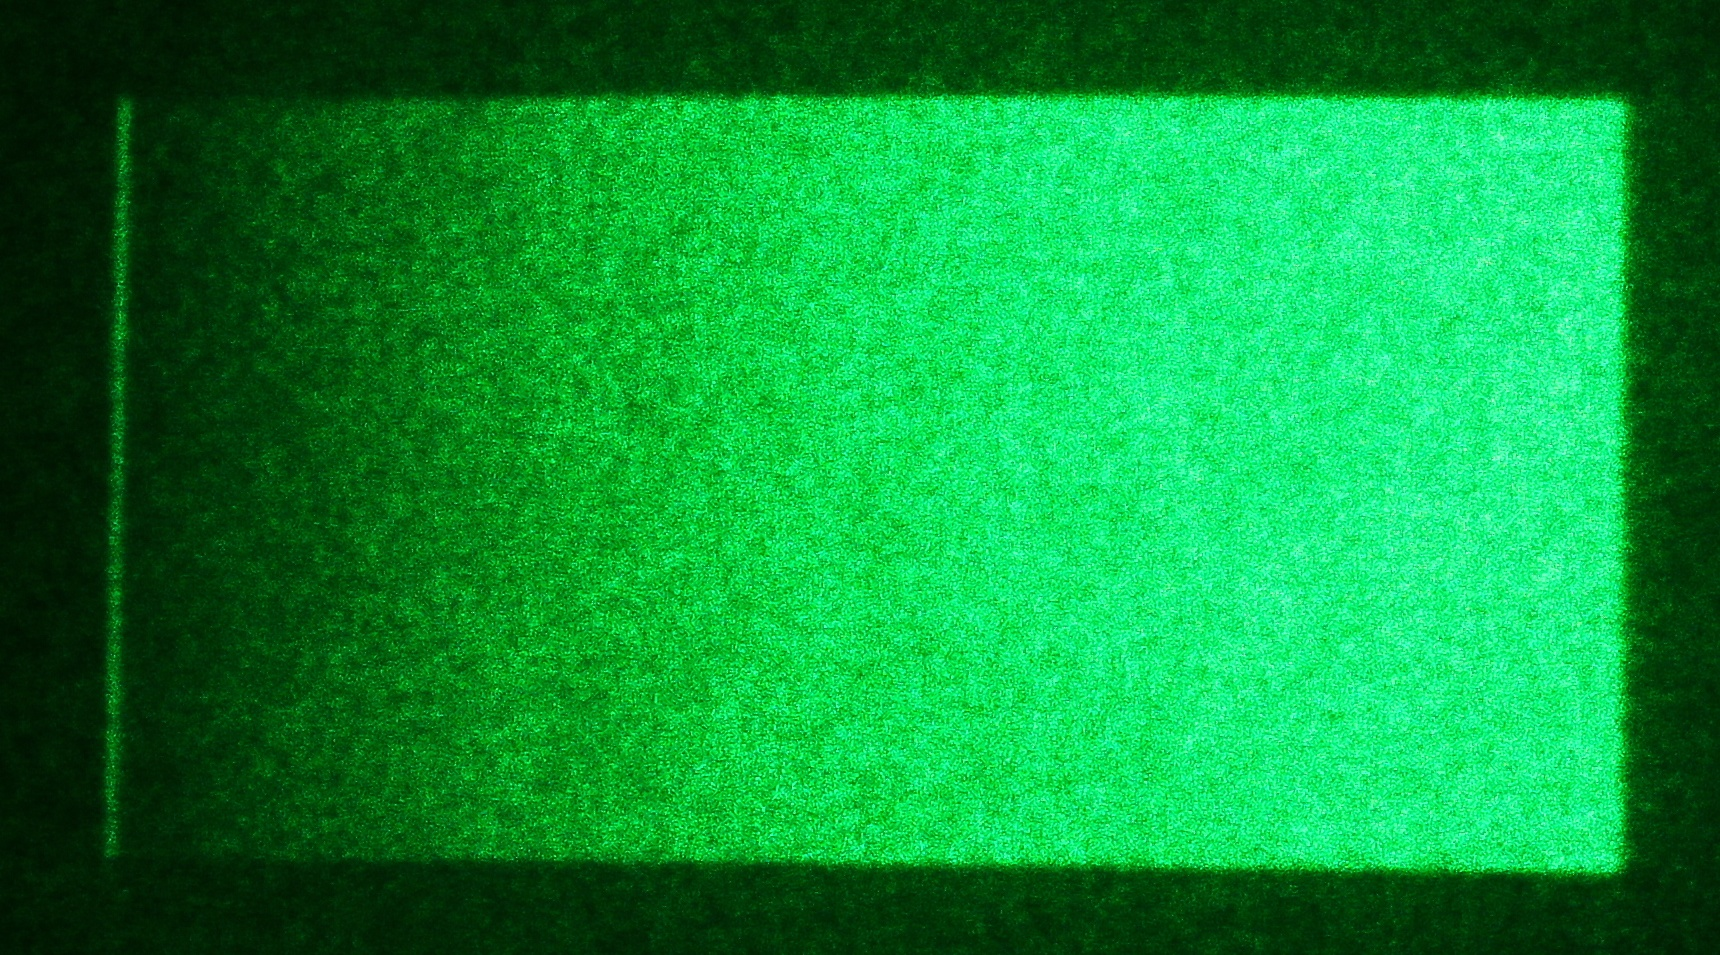
\includegraphics[width=\textwidth]{Replay field of holographic projection of linear ramp.jpg}
    \caption{Holographic projection replay field of \cref{fig:Holo_linear_ramp}}\label{fig:Replay field of holographic projection of linear ramp}
  \end{subfigure}

  \begin{subfigure}[c]{0.6\textwidth}
    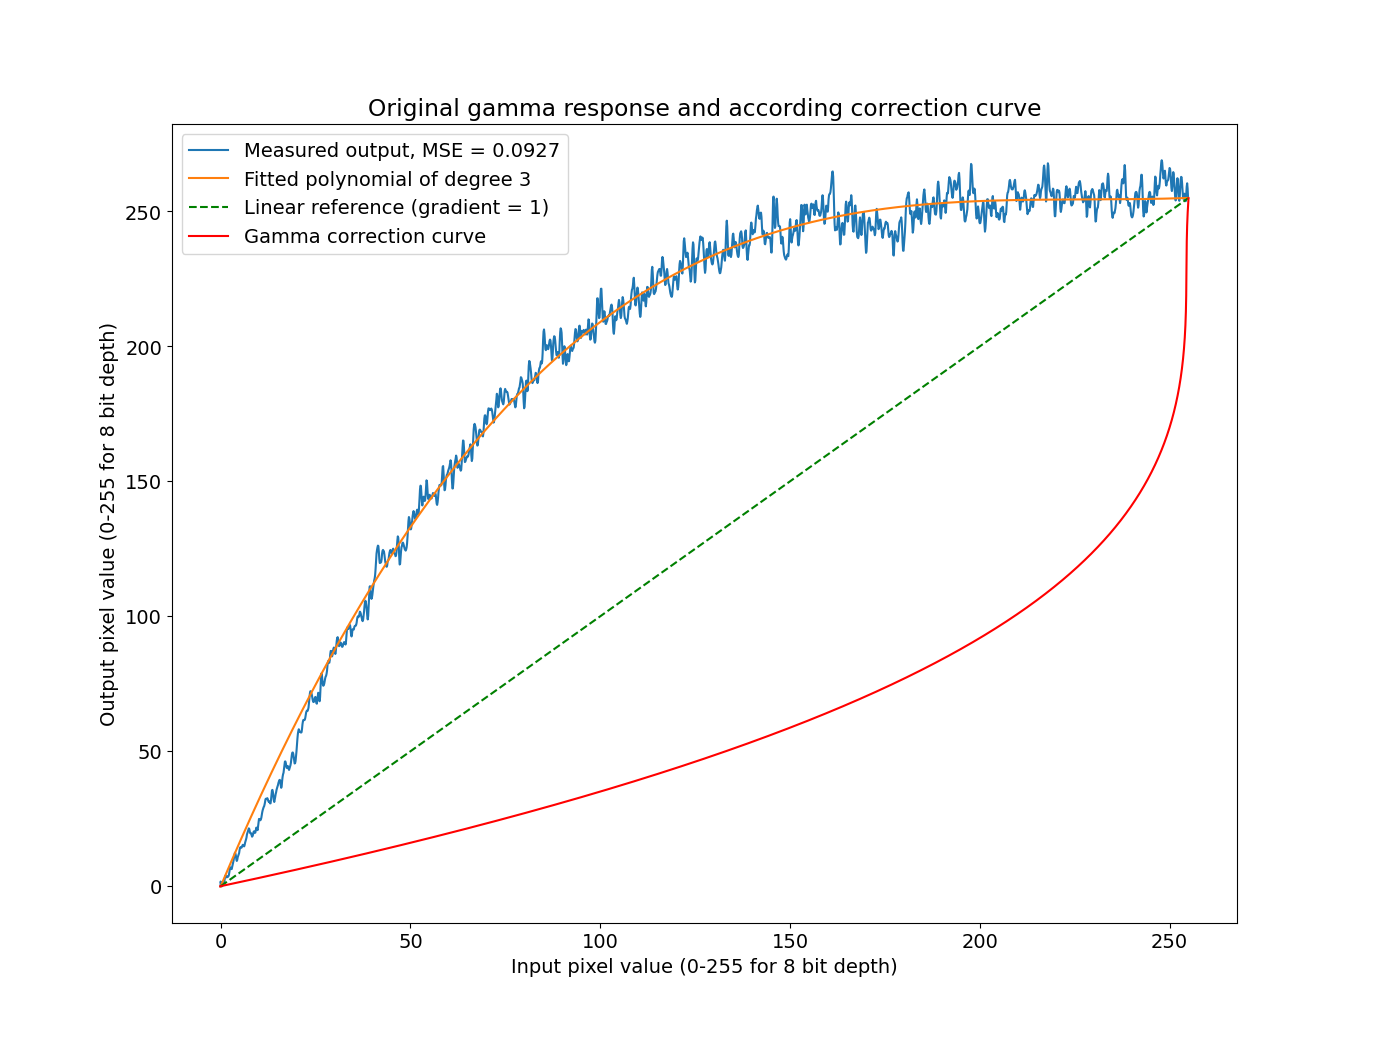
\includegraphics[width=\textwidth]{GammaResponseOriginal.png}
    \caption{Gamma response curve and according correction curve}\label{fig:GammaResponseOriginal}
  \end{subfigure}

  \caption{Measurement of gamma response, which inverse is the correction}
\end{figure}

To determine the gamma correction curve of the holographic projection system, the gamma response needs to be measured first. A hologram was generated to form a linear grey-scale ramp of brightness from 0 to 255, as shown in \cref{fig:grey-scale-test}, along with a single pixel white (255) strip at the left end as a fiducial marker to demonstrate the beginning of the grey-scale region \cite{Cable2006}.

The projection output of the linear grey-scale ramp was captured as shown in \cref{fig:Replay field of holographic projection of linear ramp}. From this the gamma response curve was determined, by averaging each column of pixels and normalising to a percentage scale, forming the blue line in \cref{fig:GammaResponseOriginal}. A three-degree polynomial fit was applied, generating a smoothed gamma response curve (yellow line in \cref{fig:GammaResponseOriginal}).

The resultant gamma response curve exhibits a high degree of non-linearity. By taking the mean of the square of the error between the measured output (blue line) and the linear reference (green dashed line), the NMSE of the measured output was calculated to be 0.0927. To correct the gamma response, the gamma correction curve (red line) was formed by inverting the gamma response curve.

\begin{figure}[H]
  \centering
  \begin{subfigure}[c]{0.32\textwidth}
    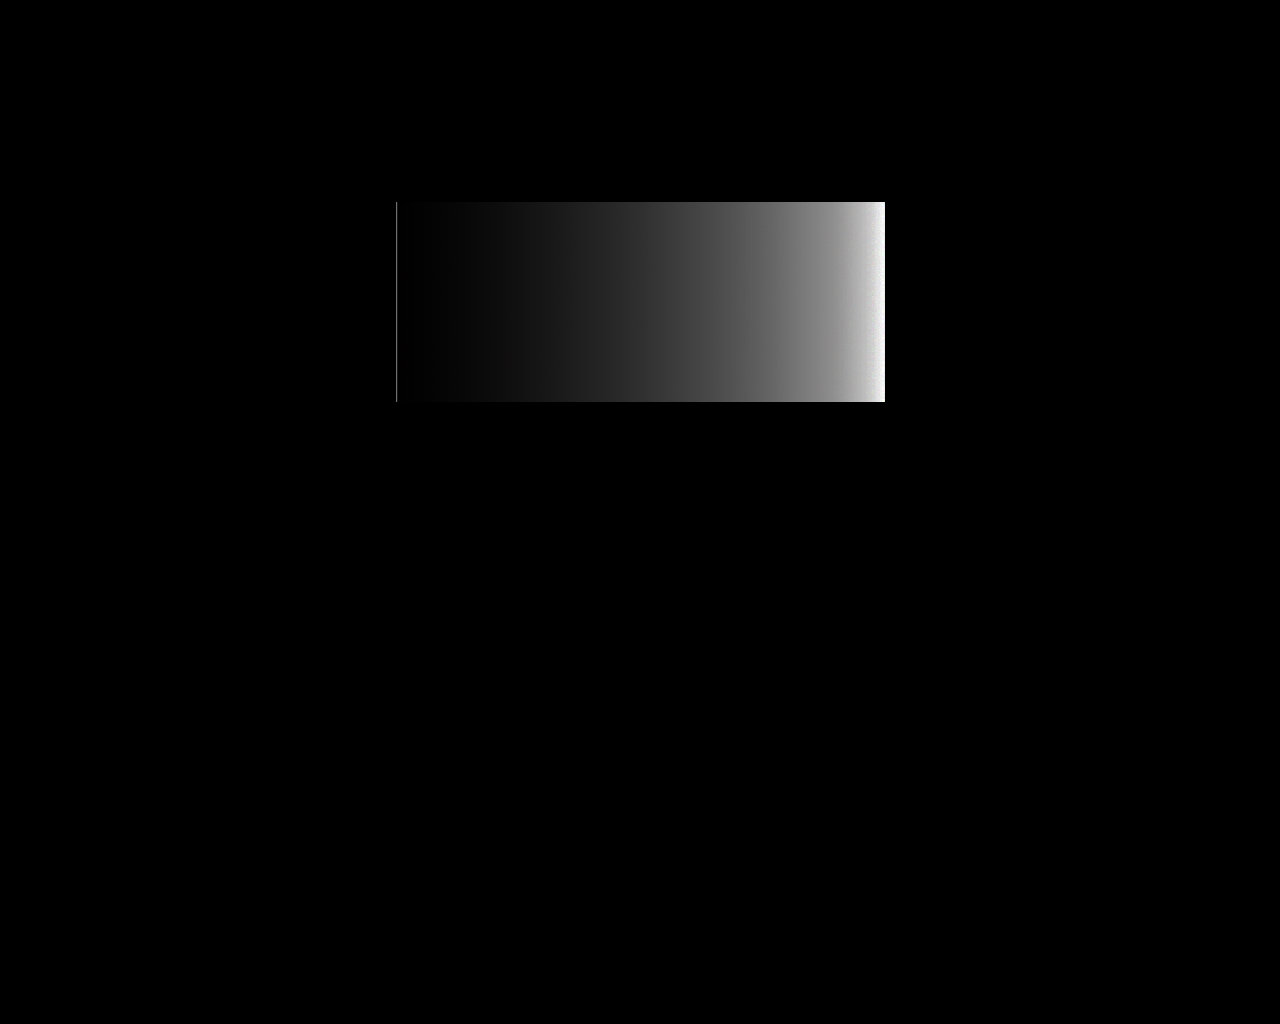
\includegraphics[width=\textwidth]{grey_scale_gamma_corrected.png}
    \caption{Input gamma corrected ramp}\label{fig:grey_scale_gamma_corrected}
  \end{subfigure}
  \hfill
  \begin{subfigure}[c]{0.32\textwidth}
    
\includegraphics[width=\textwidth]{Holo_gamma_corrected_ramp.png}
    \caption{CGH of \cref{fig:grey_scale_gamma_corrected}}\label{fig:Holo_gamma_corrected_ramp}
  \end{subfigure}
  \hfill
  \begin{subfigure}[c]{0.32\textwidth}
    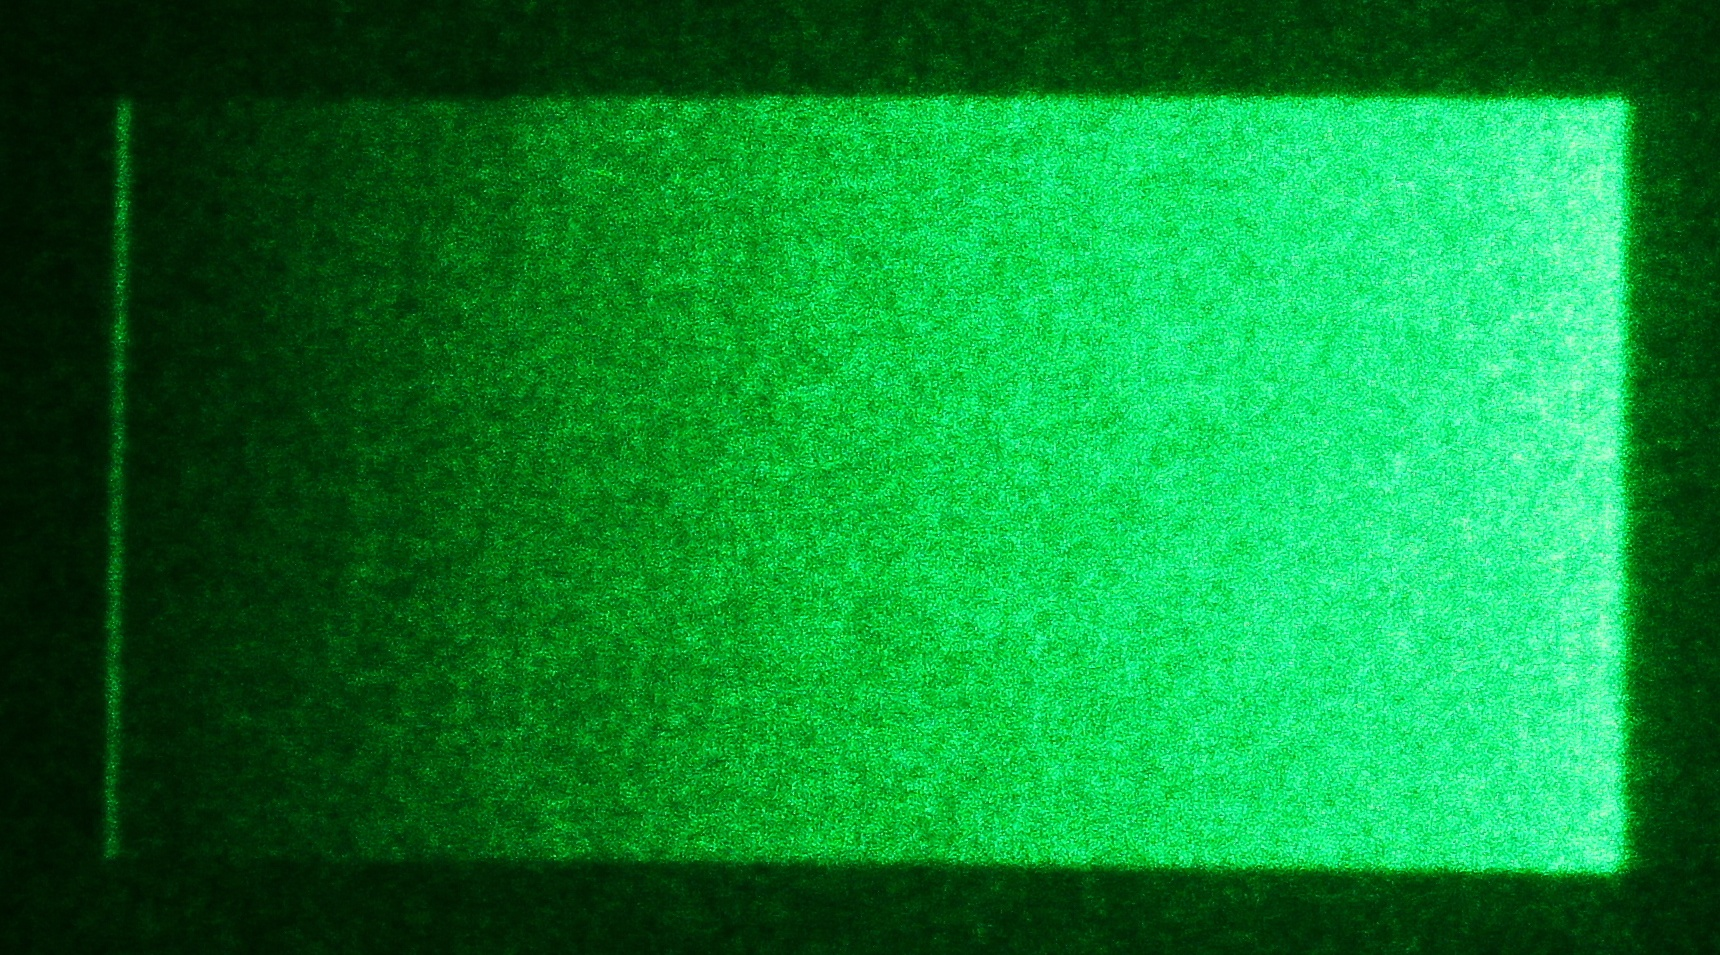
\includegraphics[width=\textwidth]{Replay field of holographic projection of gama corrected ramp.jpg}
    \caption{Holographic projection replay field of \cref{fig:Holo_gamma_corrected_ramp}}\label{fig:Replay field of holographic projection of gama corrected ramp}
  \end{subfigure}

  \begin{subfigure}[t]{0.6\textwidth}
    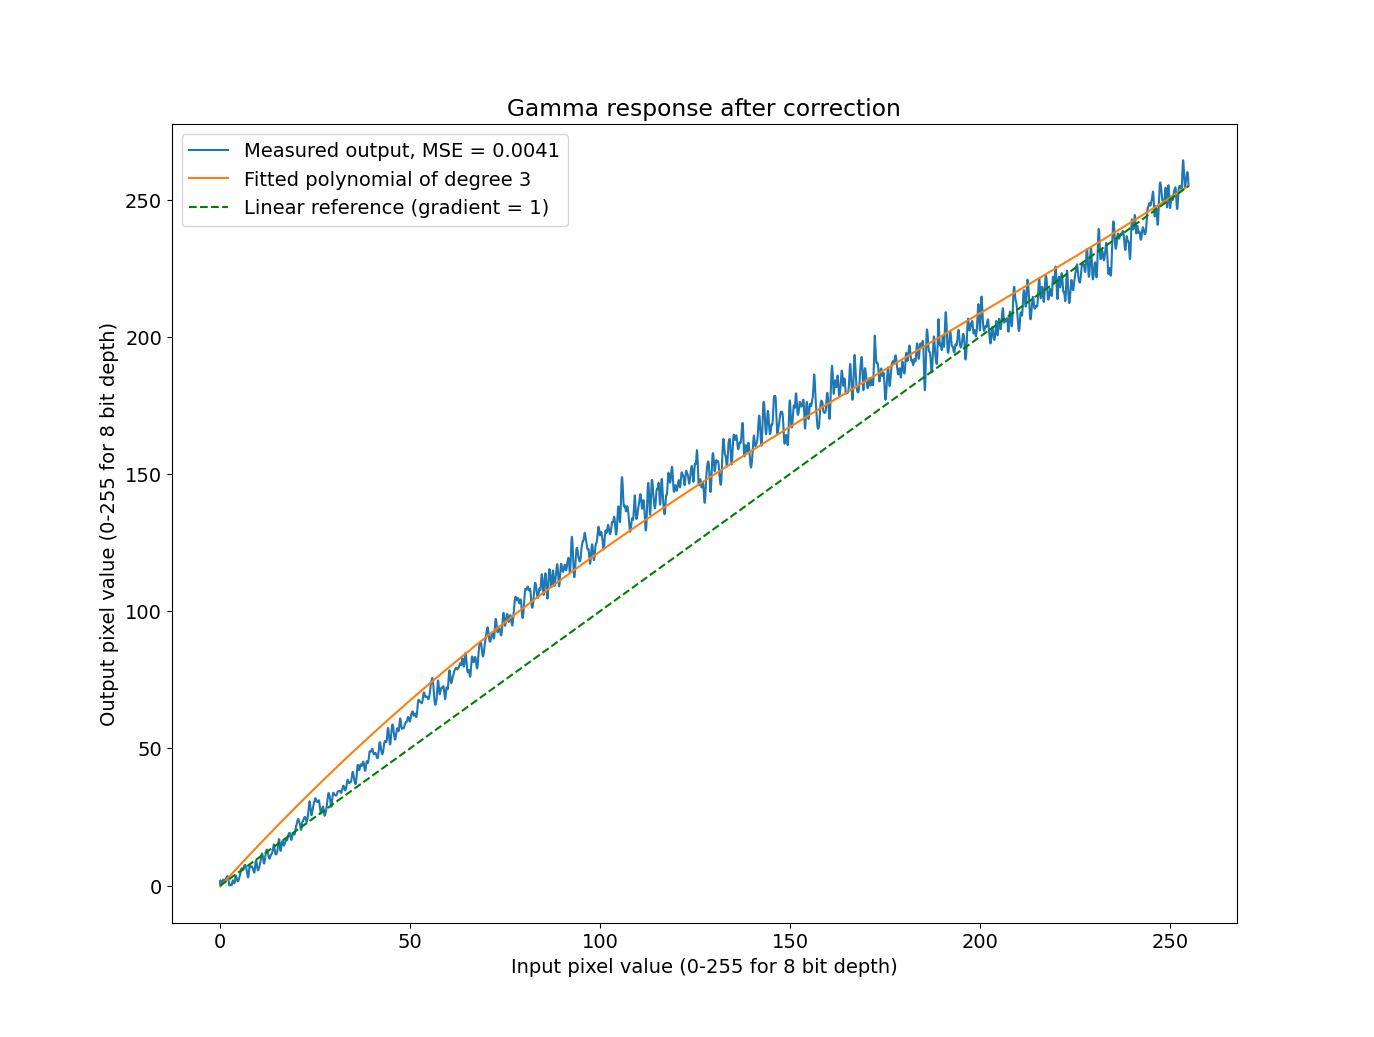
\includegraphics[width=\textwidth]{GammaResponseCorrected.png}
    \caption{Gamma response curve after correction}\label{fig:GammaResponseCorrected}
  \end{subfigure}

  \caption{Application of the correction curve on the grey-scale ramp}
\end{figure}

Subsequently, the gamma correction curve was implemented to adjust the grey-scale ramp, achieving the gamma corrected grey-scale ramp as shown in \cref{fig:grey_scale_gamma_corrected}. The gamma corrected projection output was captured as shown in \cref{fig:Replay field of holographic projection of gama corrected ramp}. By using the same method of averaging columns of pixels, the gamma corrected output was measured and plotted in \cref{fig:GammaResponseCorrected}. It can be seen that the corrected gamma response was much closer to linear comparing to the original gamma response, and the NMSE was calculated to be 0.0041.

\begin{table}[H]
  \caption{Gamma response results before and after gamma correction}
  \centering
  \label{tab:Gamma response result}
  \begin{tabular}{lll}
    \toprule
                                     & NMSE   & Percentage \\
    \midrule
    Gamma response before correction & 0.0927 & 100\%      \\
    Gamma response after correction  & 0.0041 & 4.42\%     \\
    \bottomrule
  \end{tabular}
\end{table}
Hence, as demonstrated in \cref{tab:Gamma response result}, gamma correction achieved a 95.58\% reduction in MSE, which was a significant improvement, proving the effectiveness of gamma correction method on the grey-scale ramp.





\section{Applying the Gamma Correction Curve}
\begin{figure}[H]
  \centering
  \begin{subfigure}[t]{0.3\textwidth}
    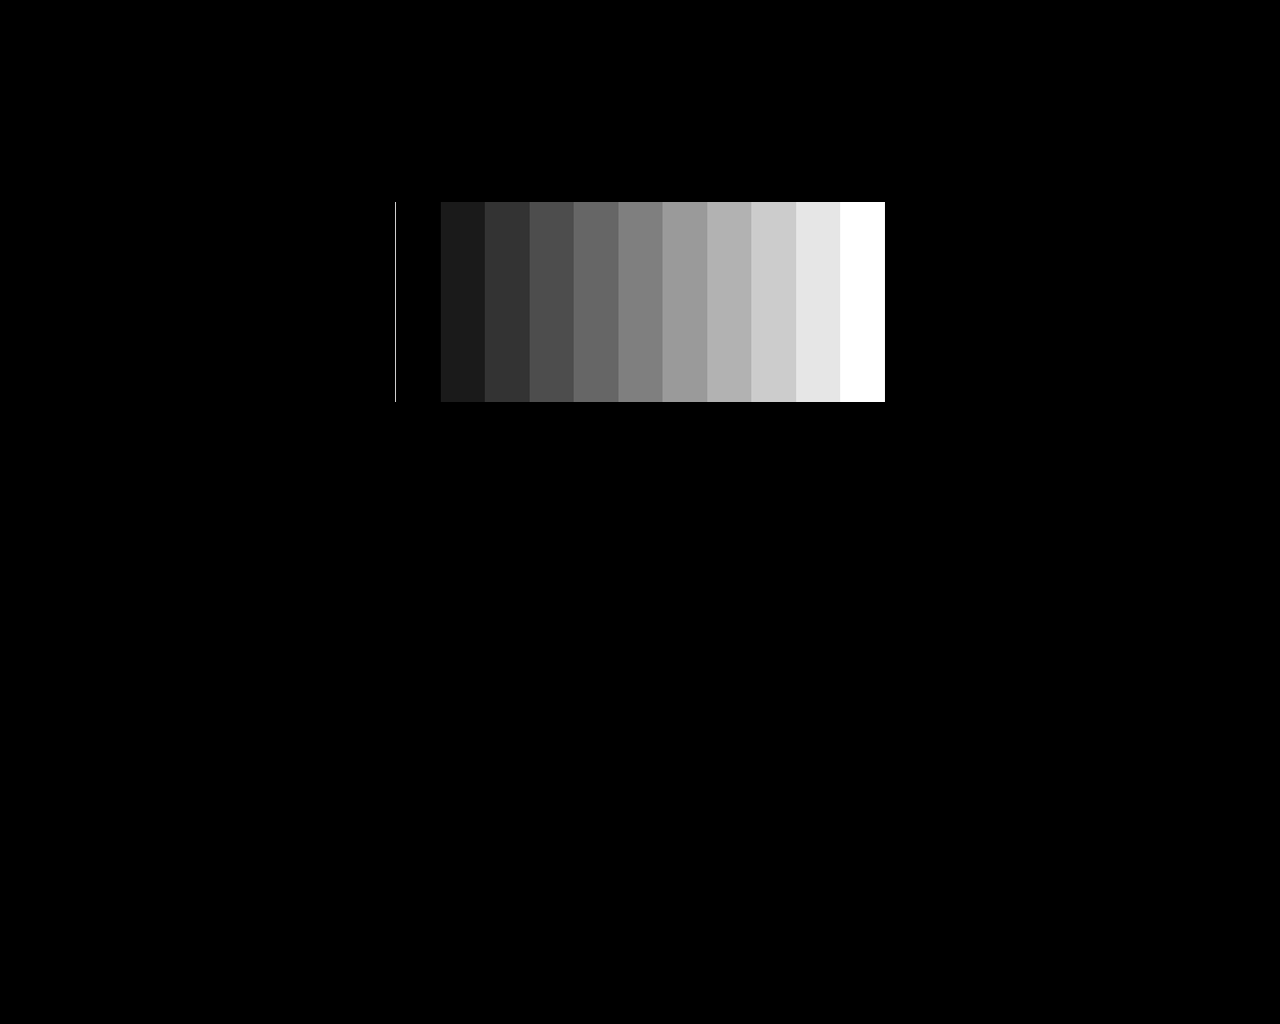
\includegraphics[width=\textwidth]{10_step_original.png}
    \caption{10 strips with equal step of pixel value}\label{fig:10_step_original}
  \end{subfigure}
  \hfill
  \begin{subfigure}[t]{0.3\textwidth}
    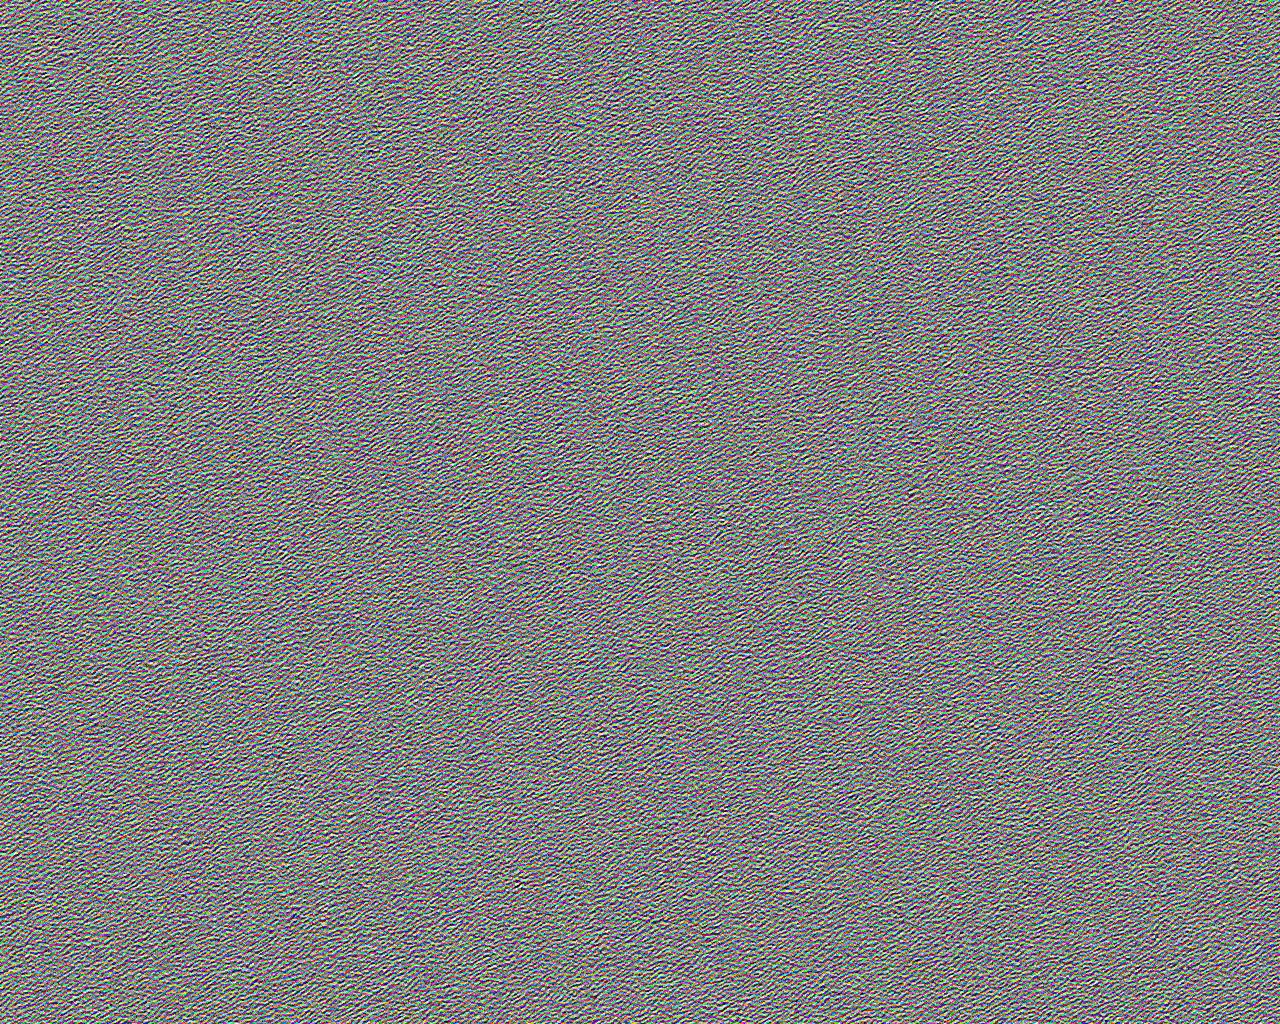
\includegraphics[width=\textwidth]{Holo_10_step_original.png}
    \caption{CGH of (a)}\label{fig:Holo_10_step_original}
  \end{subfigure}
  \hfill
  \begin{subfigure}[t]{0.37\textwidth}
    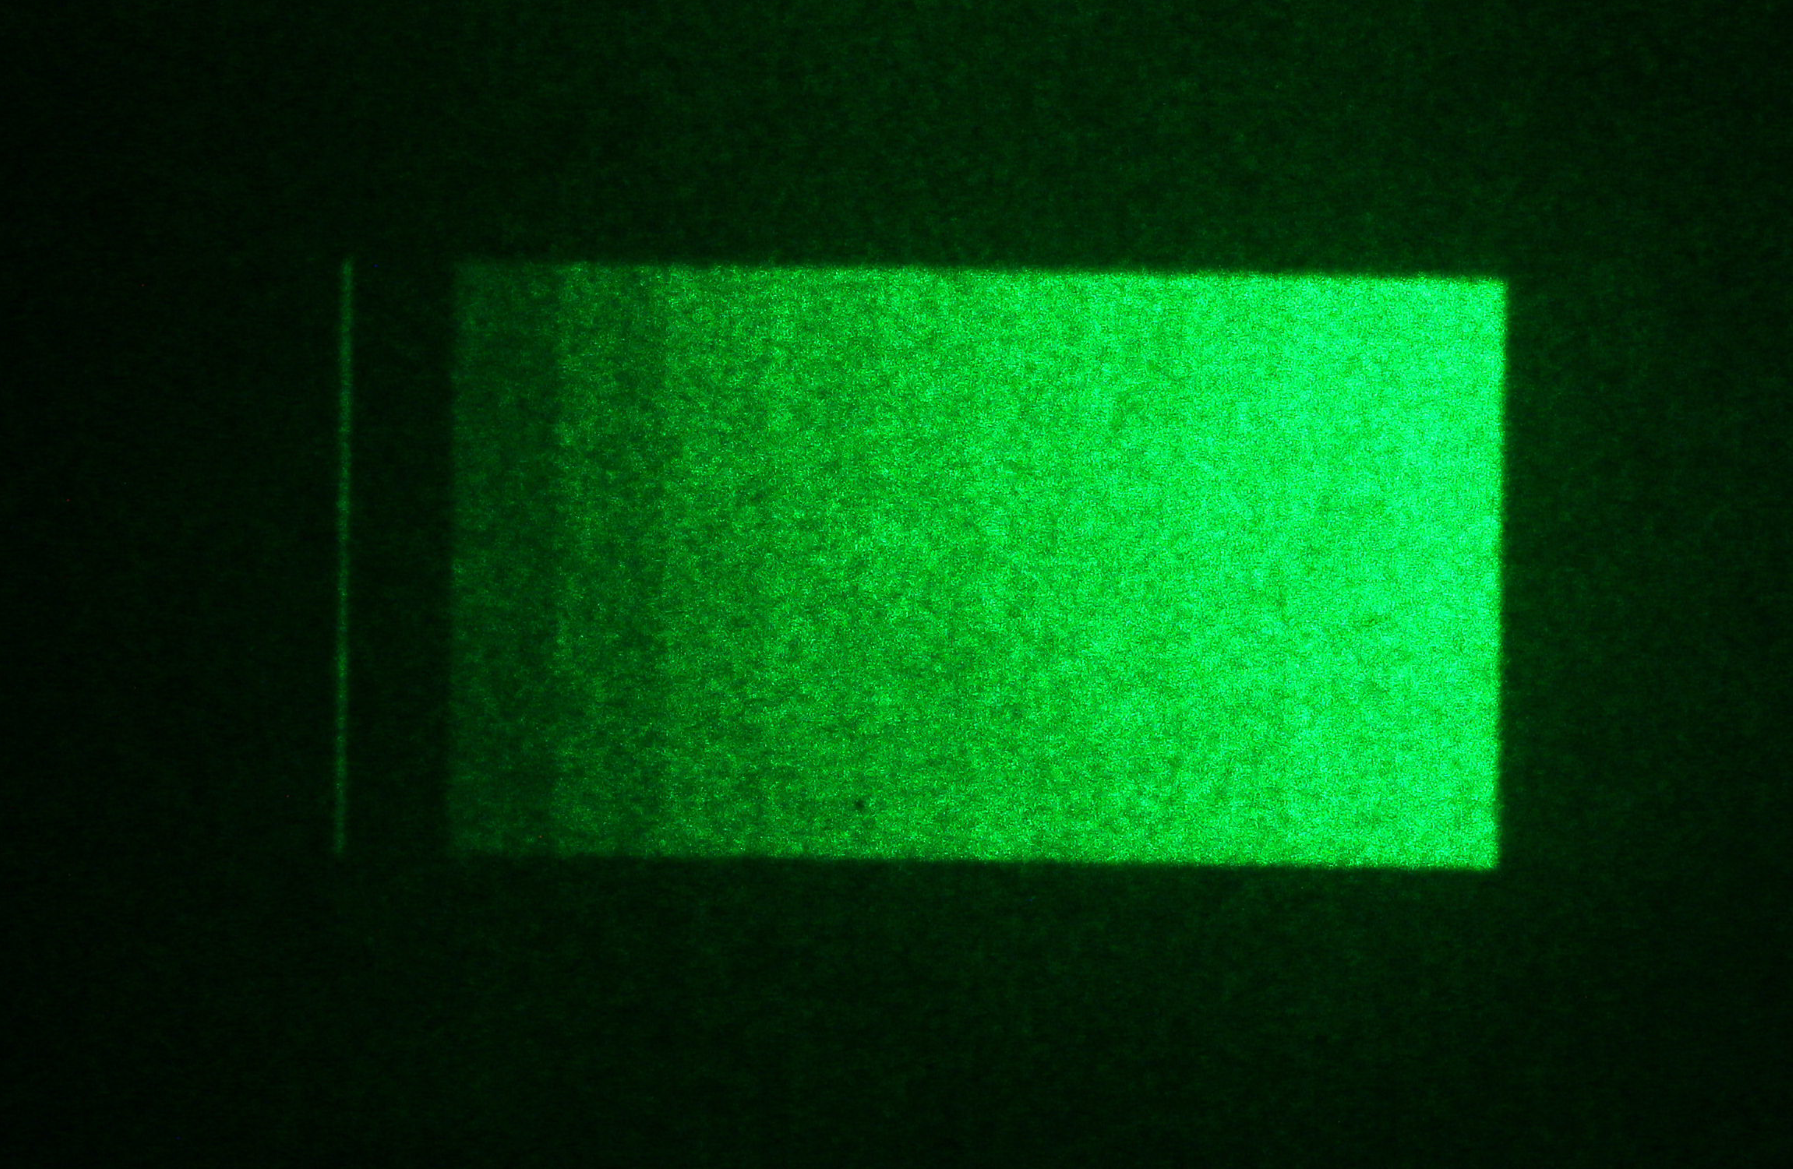
\includegraphics[width=\textwidth]{10step_before_correction.png}
    \caption{Holographic projection replay field of (b)}\label{fig:10step_before_correction}
  \end{subfigure}

  \begin{subfigure}[t]{0.3\textwidth}
    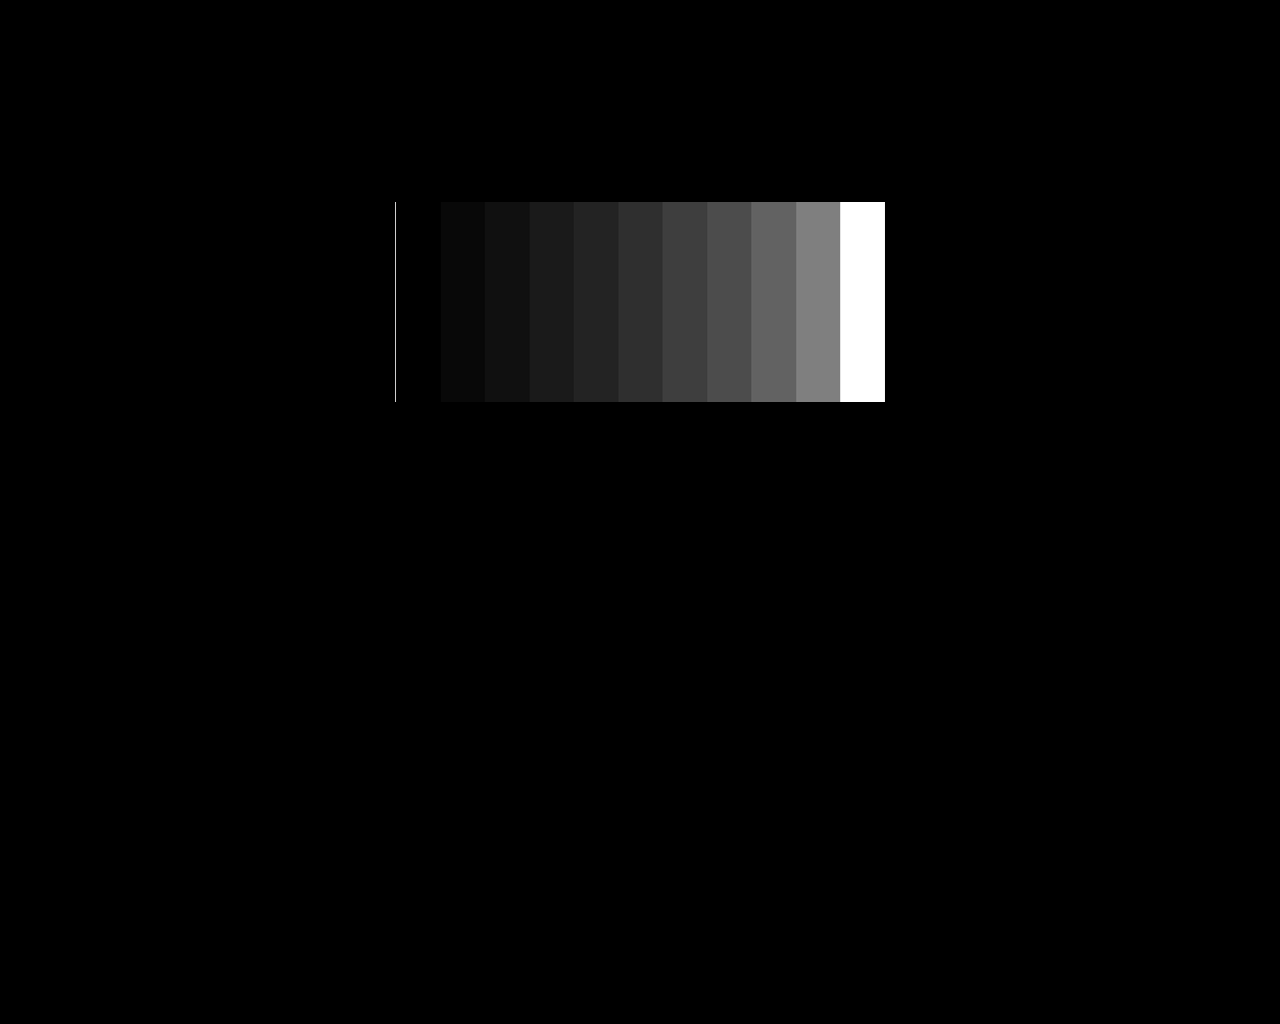
\includegraphics[width=\textwidth]{10_step_corrected.png}
    \caption{Digital pre-distortion of (a)}\label{fig:10_step_corrected}
  \end{subfigure}
  \hfill
  \begin{subfigure}[t]{0.3\textwidth}
    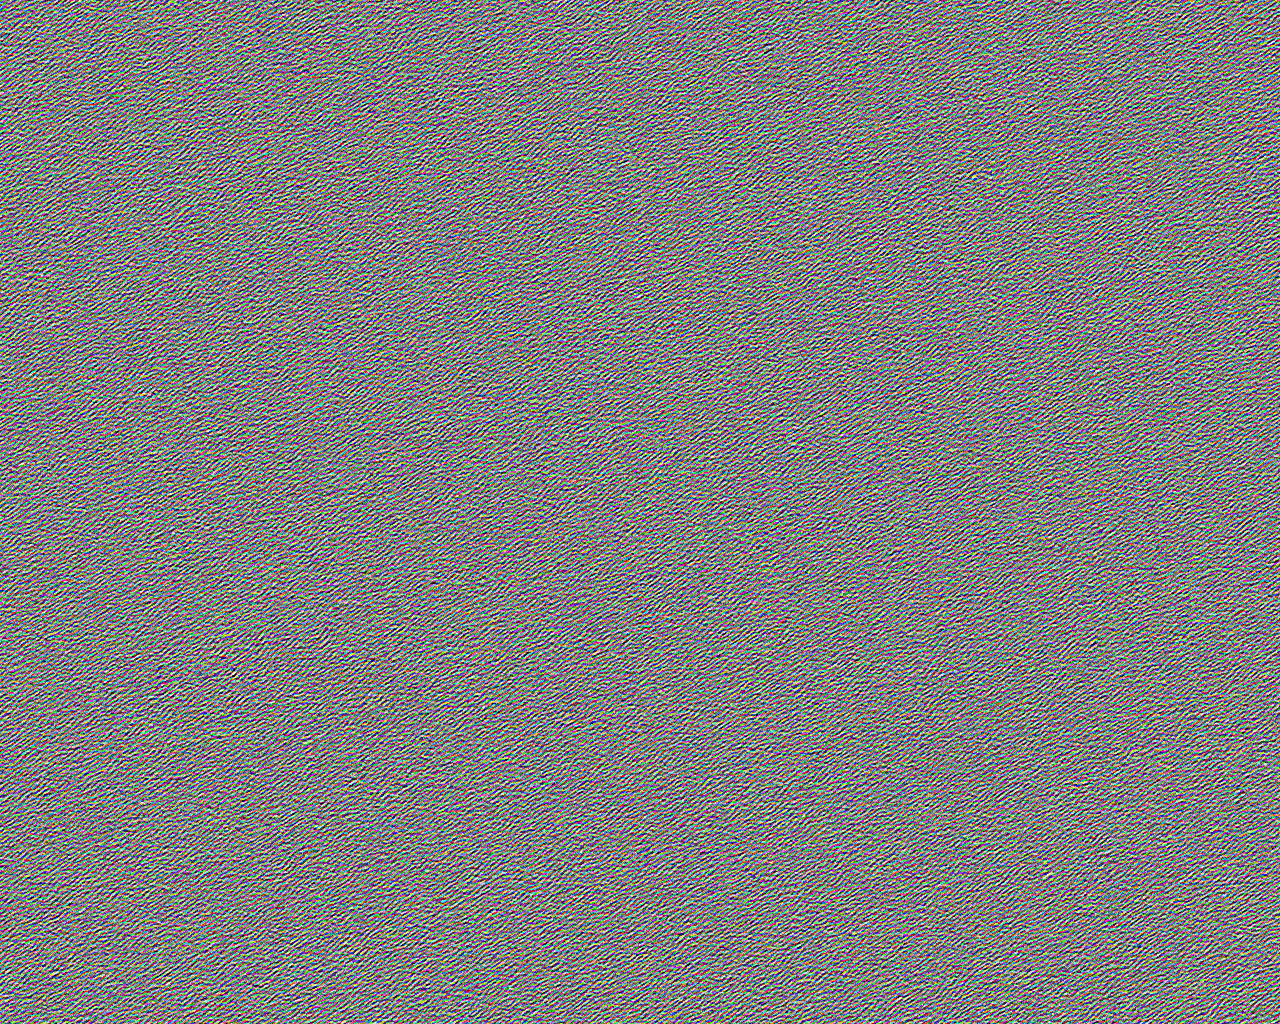
\includegraphics[width=\textwidth]{Holo_10_step_corrected.png}
    \caption{CGH of (d)}\label{fig:Holo_10_step_corrected}
  \end{subfigure}
  \hfill
  \begin{subfigure}[t]{0.37\textwidth}
    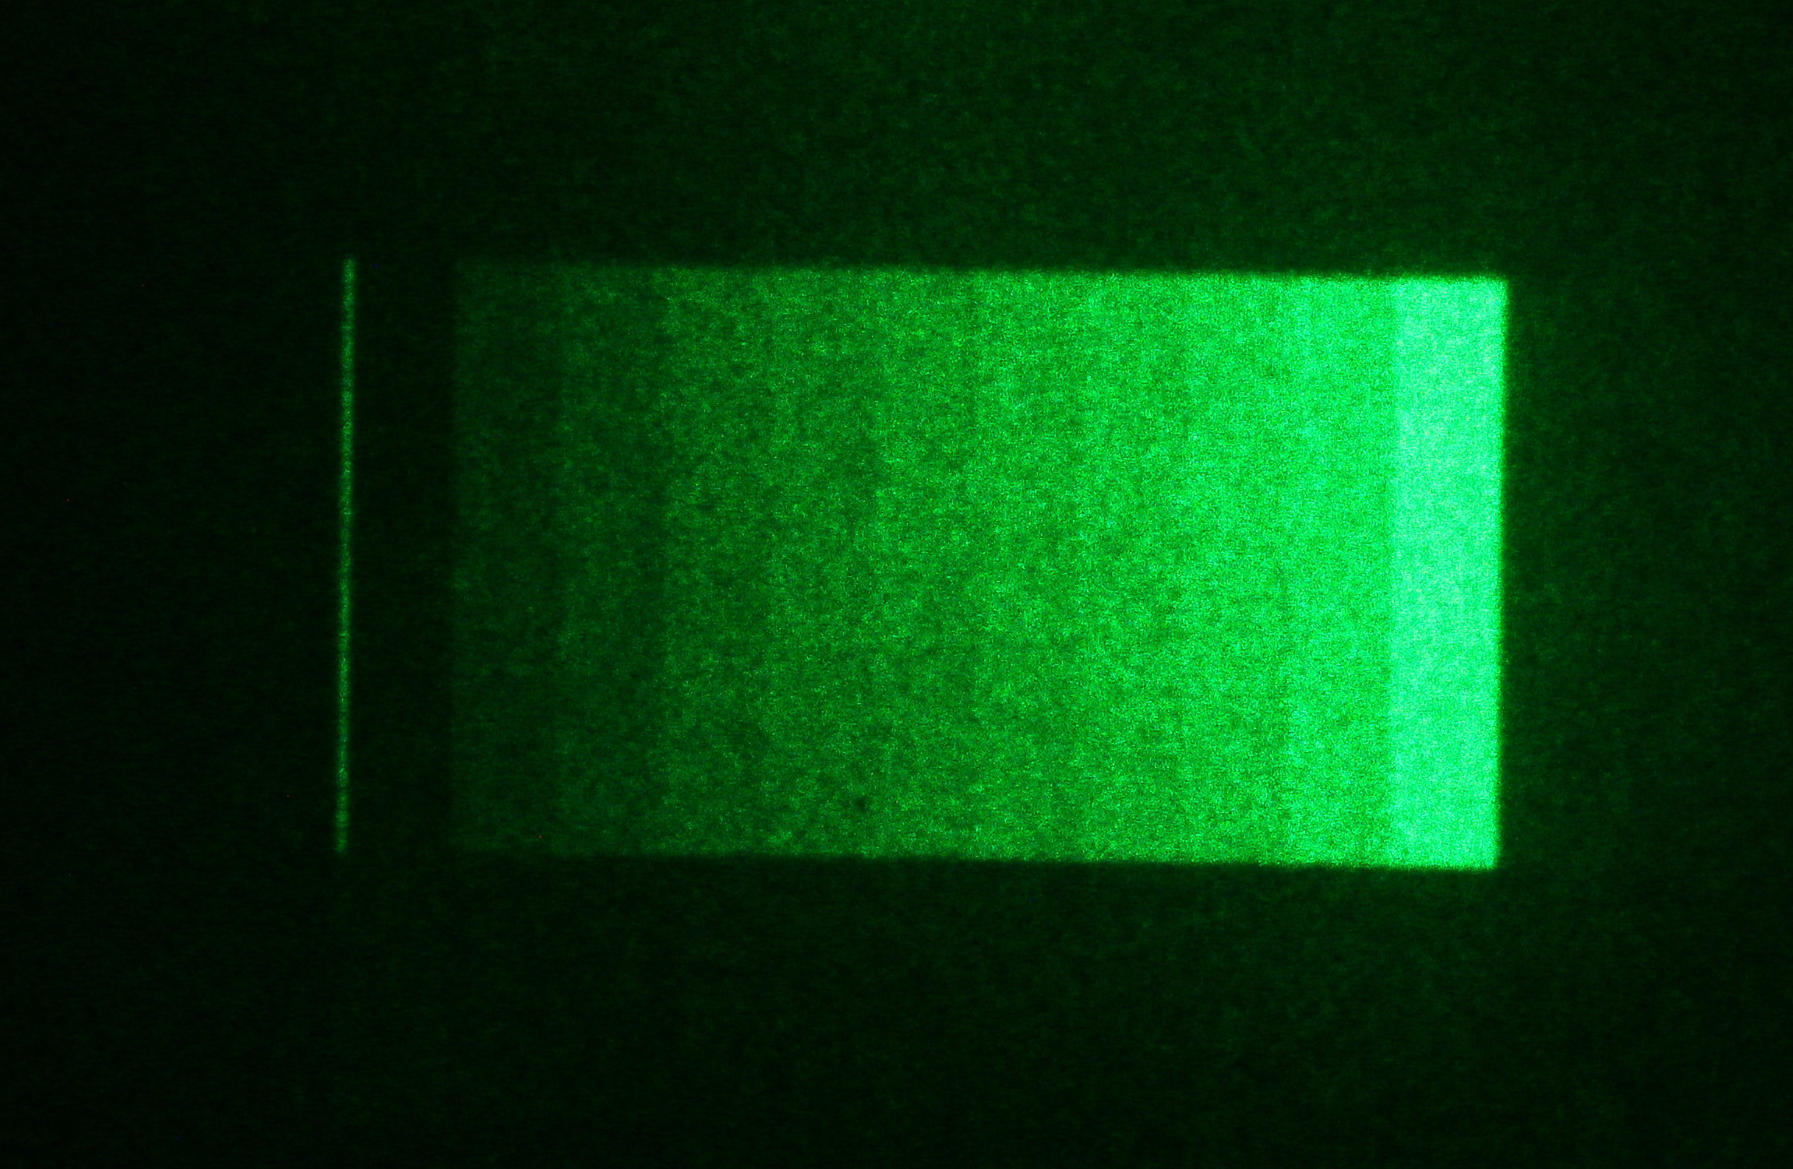
\includegraphics[width=\textwidth]{10step_after_correction.png}
    \caption{Holographic projection replay field of (f)}\label{fig:10step_after_correction}
  \end{subfigure}

  \caption{Application of the correction curve on 10-step strips}
  \label{fig:Application of the correction curve on 10-step strips}
\end{figure}

As shown in \cref{fig:Application of the correction curve on 10-step strips}, when CGH is computed for the 10 strips with equal step of pixel value \cref{fig:10_step_original}, the right few strips in \cref{fig:10step_before_correction} are barely distinguishable. After applying the correction curve obtained in \cref{sec:Determining the gamma correction curve}, it can be seen that each pair of adjacent strips in \cref{fig:10step_after_correction} are much more distinguishable, validating the effectiveness of the gamma correction method.


\begin{figure}[H]
  \centering
  \begin{subfigure}[t]{0.4\textwidth}
    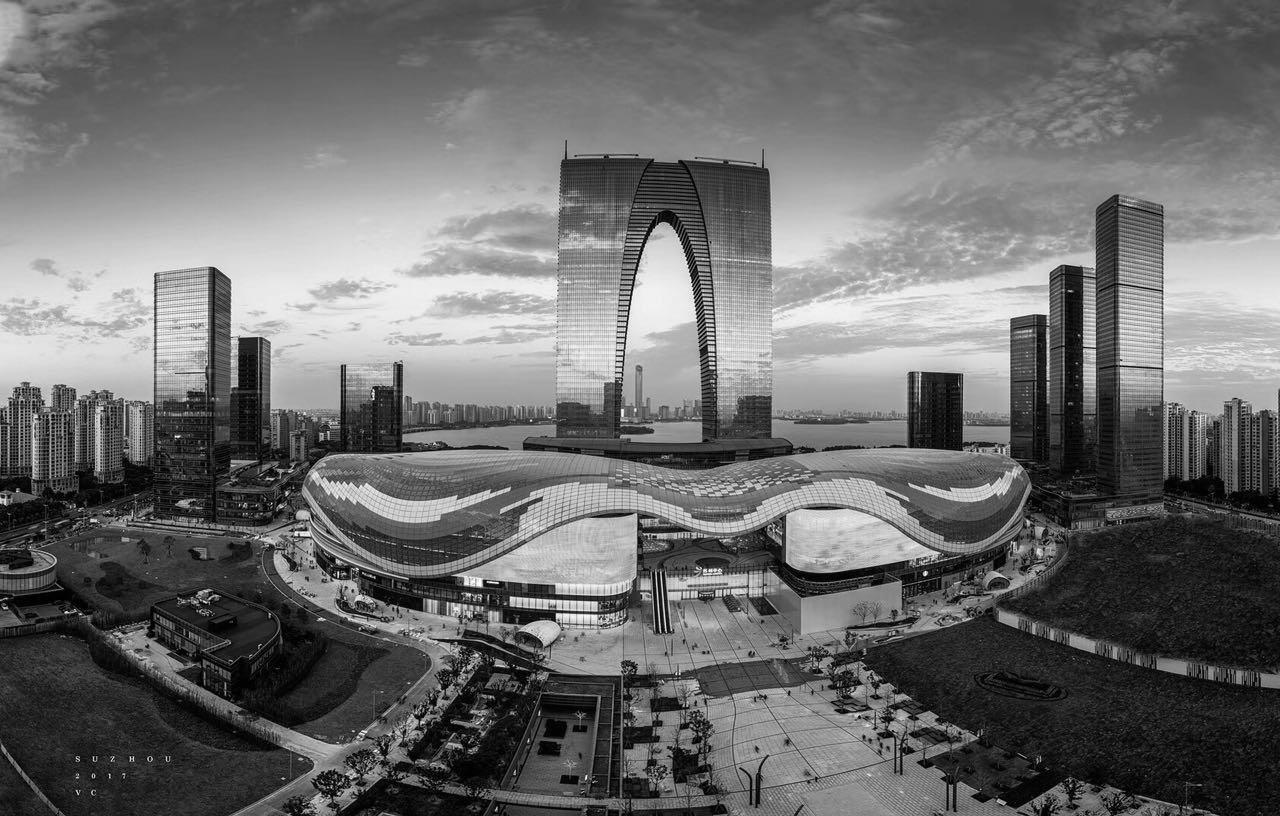
\includegraphics[width=\textwidth]{szzx_grey.jpg}
    \caption{Sample image 1: City Scene \cite{Zhao2017}}\label{fig:szzx_grey}
  \end{subfigure}
  \quad
  \begin{subfigure}[t]{0.219\textwidth}
    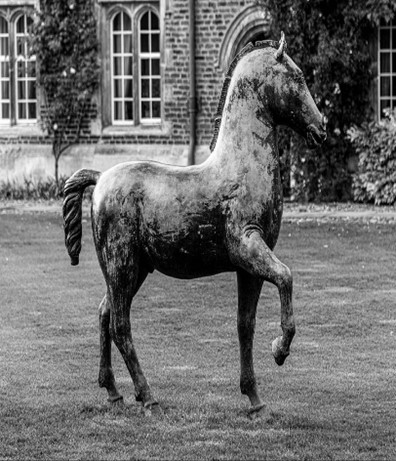
\includegraphics[width=\textwidth]{horse_grey.jpg}
    \caption{Sample image 2: Horse}\label{fig:horse_grey}
  \end{subfigure}

  \begin{subfigure}[t]{0.4\textwidth}
    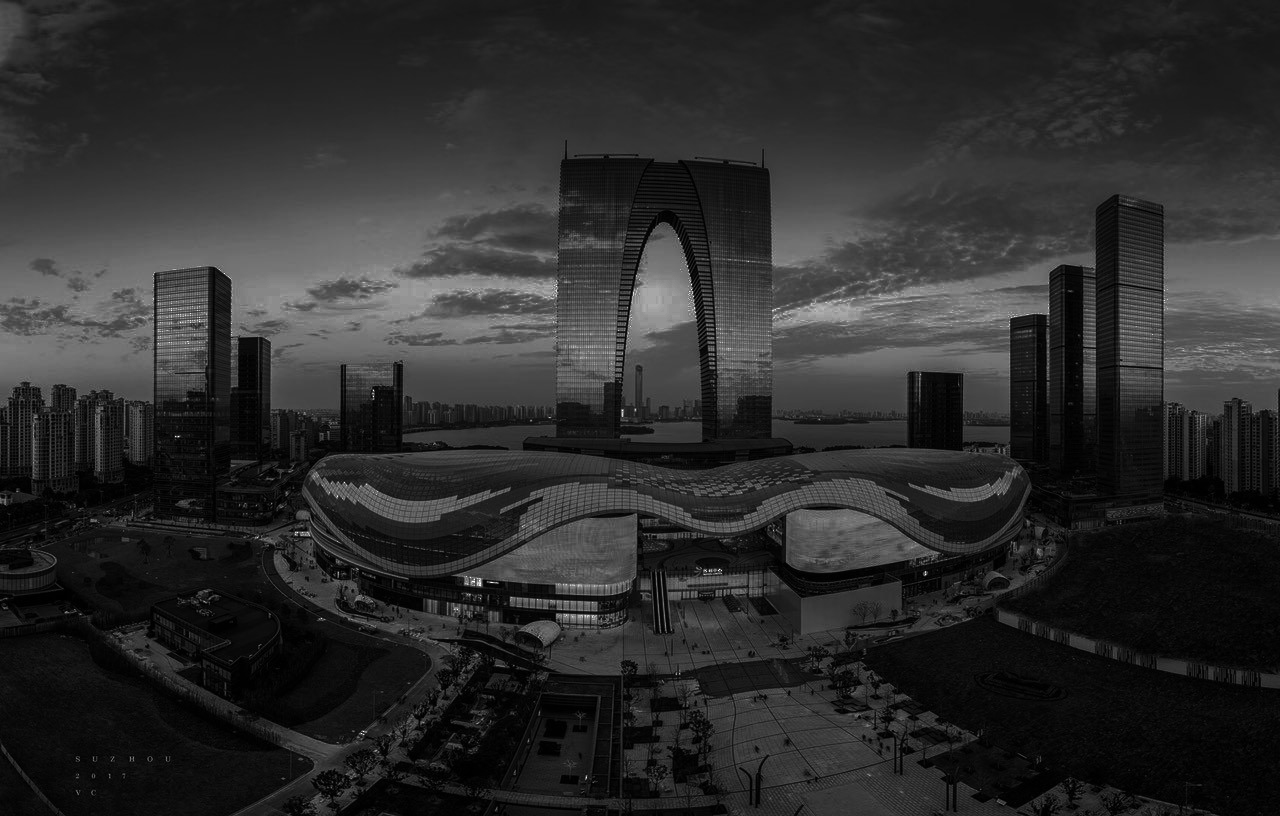
\includegraphics[width=\textwidth]{szzx_grey_gamma_corrected.jpg}
    \caption{Sample image 1 after gamma correction}\label{fig:szzx_grey_gamma_corrected}
  \end{subfigure}
  \quad
  \begin{subfigure}[t]{0.219\textwidth}
    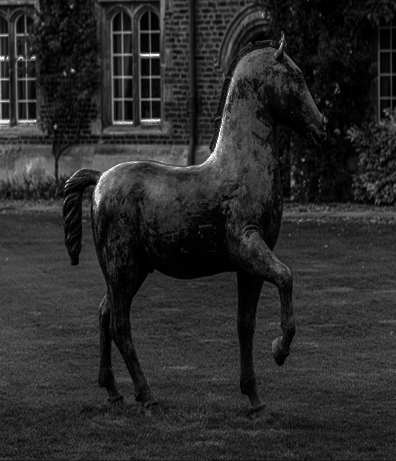
\includegraphics[width=\textwidth]{horse_grey_gamma_corrected.jpg}
    \caption{Sample image 2 after gamma correction}\label{fig:horse_grey_gamma_corrected}
  \end{subfigure}

  \caption{Application of the correction curve on two sample real-word images}
  \label{fig:Application of the correction curve on two sample real-word images}
\end{figure}

Then the gamma correction curve was applied to the two sample images as shown in \cref{fig:Application of the correction curve on two sample real-word images}.

\begin{figure}[H]
  \centering
  \begin{subfigure}[t]{0.4\textwidth}
    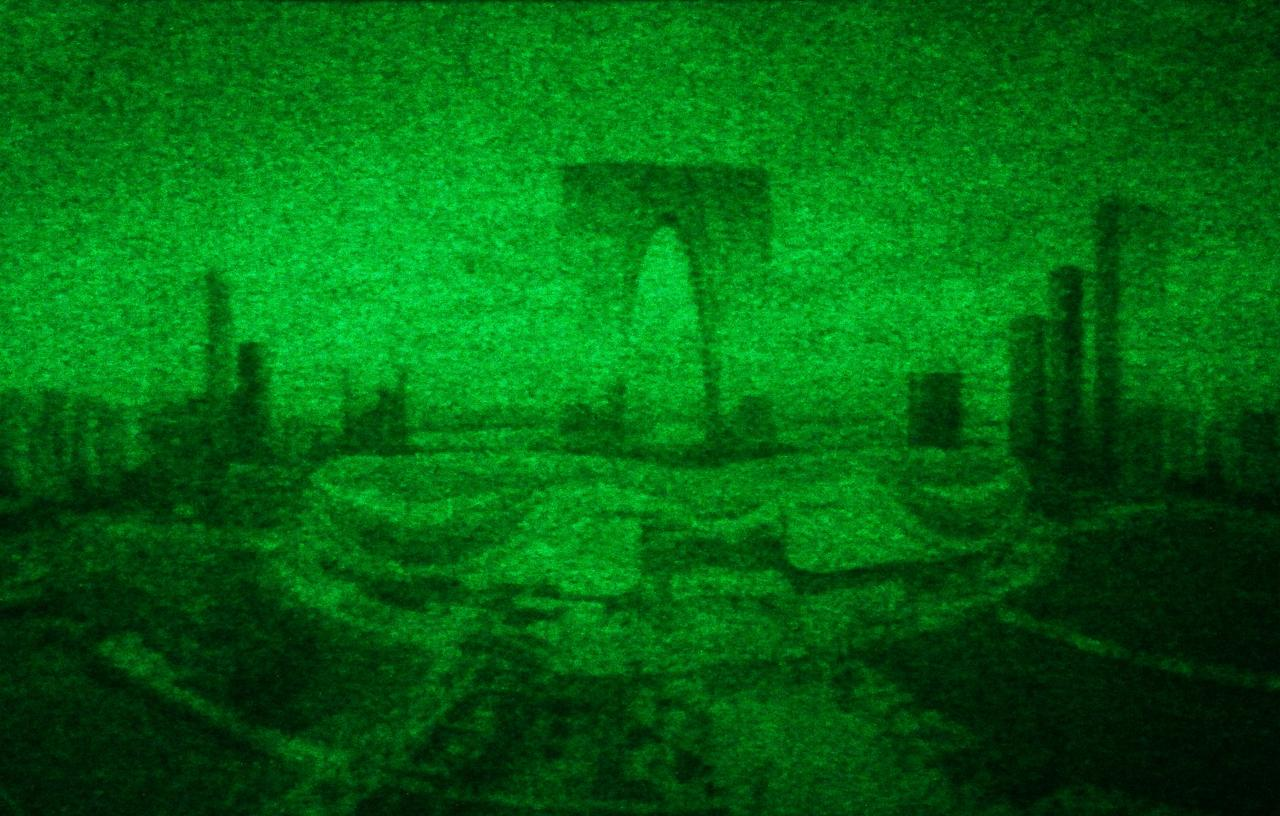
\includegraphics[width=\textwidth]{szzx_original.jpg}
    \caption{Replay field of Sample image 1 before gamma correction (NMSE=0.06139)}\label{fig:szzx_original}
  \end{subfigure}
  \quad
  \begin{subfigure}[t]{0.219\textwidth}
    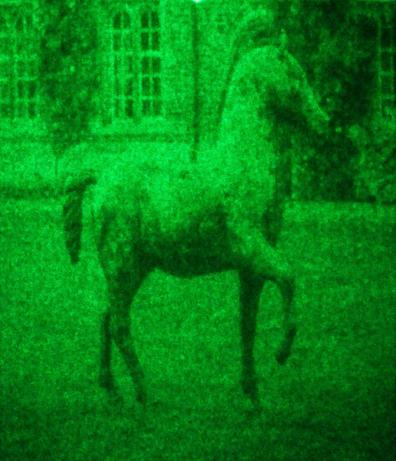
\includegraphics[width=\textwidth]{horse_original.jpg}
    \caption{Replay field of Sample image 2 before gamma correction (NMSE=0.04309)}\label{fig:horse_original}
  \end{subfigure}

  \begin{subfigure}[t]{0.4\textwidth}
    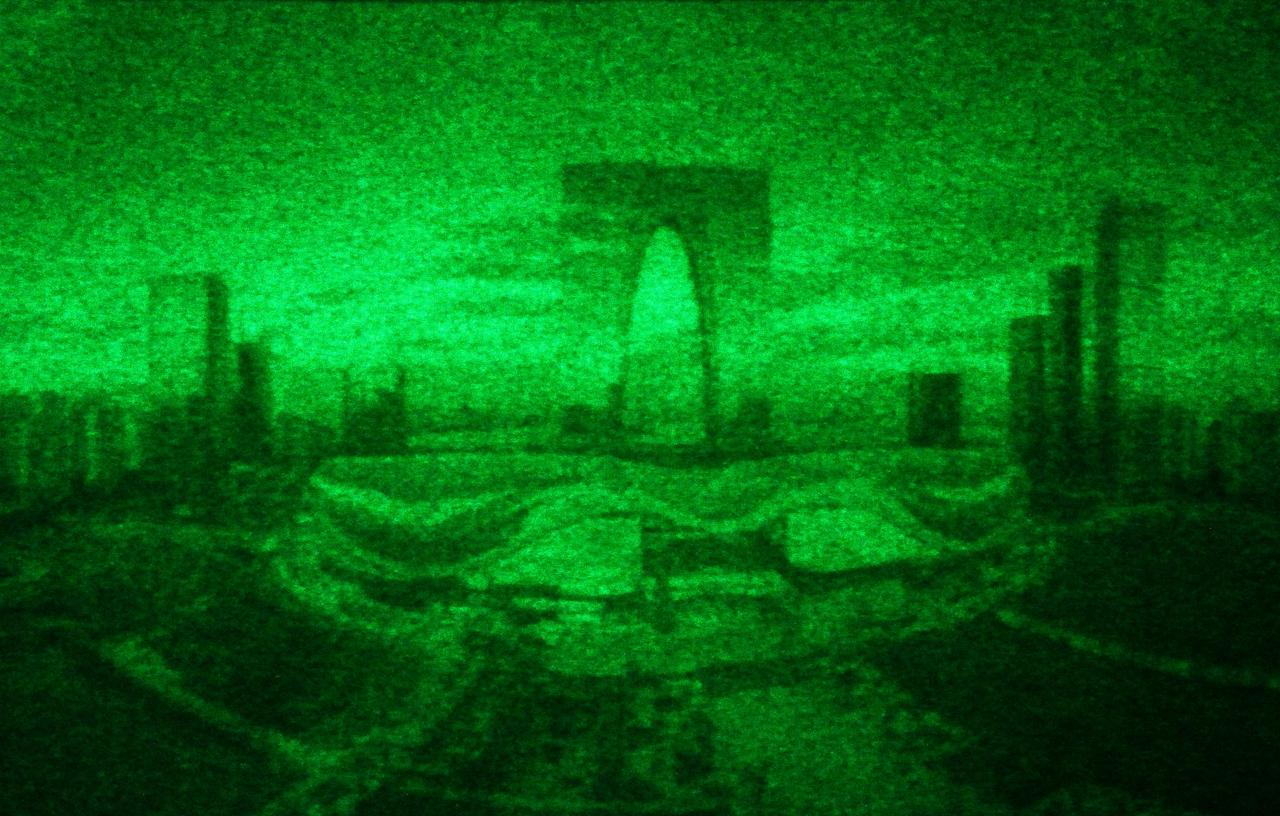
\includegraphics[width=\textwidth]{szzx_gamma_corrected.jpg}
    \caption{Replay field of Sample image 1 after gamma correction (NMSE=0.04920)}\label{fig:szzx_gamma_corrected}
  \end{subfigure}
  \quad
  \begin{subfigure}[t]{0.219\textwidth}
    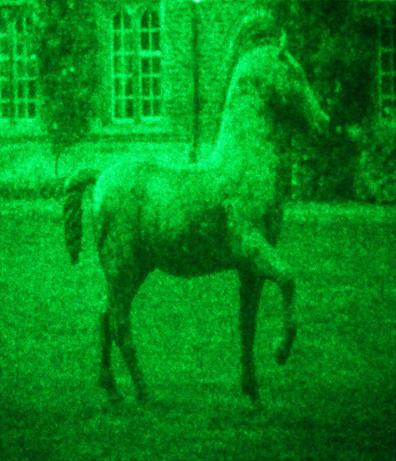
\includegraphics[width=\textwidth]{horse_gamma_corrected.jpg}
    \caption{Replay field of Sample image 2 after gamma correction (NMSE=0.03635)}\label{fig:horse_gamma_corrected}
  \end{subfigure}

  \caption{Projection output of the two sample images before and after gamma correction}
\end{figure}

The replay fields of the holographic projection of uncorrected images are shown in \cref{fig:szzx_original} and \cref{fig:horse_original}, and the replay fields of the holographic projection of images after gamma correction are shown in \cref{fig:szzx_gamma_corrected} and \cref{fig:horse_gamma_corrected} respectively.

As shown in \cref{fig:szzx_original}, it can be seen that, before gamma correction, the edges between the buildings and the sky were quite ambiguous, with most detail of the sky being lost. In comparison, after gamma correction, the replay field in \cref{fig:szzx_gamma_corrected} provided not only sharper edges between buildings and the sky, but also more detail of clouds in the sky. The NMSE of the replay field for sample image 1 decreased from 0.06139 to 0.04920, which was a 19.86\% reduction.

In \cref{fig:horse_original}, before gamma correction, the horse was difficult to distinguish from the background, especially around the horse's back area. But after gamma correction, as shown in \cref{fig:horse_gamma_corrected}, contrast has been significantly boosted and the fine detail around this part of the horse is more evident. The NMSE of the replay field for sample image 2 decreased from 0.04309 to 0.03635, which was a 15.64\% reduction.

\begin{table}[H]
  \caption{Gamma correction results for sample images}
  \centering
  \label{tab:Gamma correction results for sample images}
  \begin{tabular}{lll}
    \toprule
    Sample image 1          & NMSE    & Percentage \\
    \midrule
    Before gamma correction & 0.06139 & 100\%      \\
    After gamma correction  & 0.04920 & 80.15\%    \\
    \midrule
    \midrule
    Sample image 2          & NMSE    & Percentage \\
    \midrule
    Before gamma correction & 0.04309 & 100\%      \\
    After gamma correction  & 0.03635 & 84.36\%    \\
    \bottomrule
  \end{tabular}
\end{table}

Hence, as summarised in \cref{tab:Gamma correction results for sample images}, gamma correction achieved a 19.86\% reduction in NMSE for sample image 1 and a 15.64\% reduction in NMSE for sample image 2, proving the effectiveness of gamma correction method on real-world test images.



\section{Summary}
The gamma response of holographic projection can exhibit a high degree of non-linearity. By projecting a linear grey-scale ramp, the gamma response of the holographic projection system was measured. The gamma correction curve, which was simply the inverse of gamma response, was applied to the grey-scale ramp and successfully reduced the NMSE by 95.58\%. And then the gamma correction method was applied on two sample images, it was observed that more details were shown in the replay field after gamma correction, and the NMSE's of the two example images were reduced by 19.86\% and 15.64\%. Hence, we have demonstrated the effectiveness of gamma correction method to boost image quality for a holographic projection system.